% Fig 2 (fig:quadtree): standalone source for the paper figure.
% Build: pdflatex quadtree.tex  ->  quadtree.pdf  (see build_figures.sh)
\documentclass[border=2pt]{standalone}
\usepackage[T1]{fontenc}
\usepackage{amsmath,amssymb}
\usepackage{tikz}
\usetikzlibrary{shapes.geometric, arrows.meta, positioning, patterns, calc}
% Okabe-Ito colorblind-safe palette (Wong 2011, Nature Methods)
\definecolor{oiblue}{HTML}{0072B2}
\definecolor{oiorange}{HTML}{E69F00}
\definecolor{oiskyblue}{HTML}{56B4E9}
\definecolor{oigray}{HTML}{999999}
\definecolor{oivermillion}{HTML}{D55E00}
\definecolor{oigreen}{HTML}{009E73}
\definecolor{oipurple}{HTML}{CC79A7}
\begin{document}
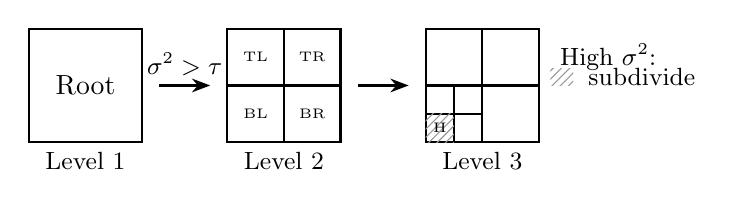
\begin{tikzpicture}[scale=0.72]
    % Initial root (left)
    \draw[thick] (0,0) rectangle (2,2);
    \node at (1,1) {Root};
    \node[below] at (1,0) {\small Level 1};

    % Arrow
    \draw[-{Stealth}, thick] (2.3,1) -- (3.2,1);
    \node[above] at (2.75,1) {\small $\sigma^2 > \tau$};

    % First subdivision (middle)
    \draw[thick] (3.5,0) rectangle (5.5,2);
    \draw[thick] (4.5,0) -- (4.5,2);
    \draw[thick] (3.5,1) -- (5.5,1);
    \node[font=\tiny] at (4,1.5) {TL};
    \node[font=\tiny] at (5,1.5) {TR};
    \node[font=\tiny] at (4,0.5) {BL};
    \node[font=\tiny] at (5,0.5) {BR};
    \node[below] at (4.5,0) {\small Level 2};

    % Arrow
    \draw[-{Stealth}, thick] (5.8,1) -- (6.7,1);

    % Final subdivision (right) - with one quadrant further subdivided
    \draw[thick] (7,0) rectangle (9,2);
    \draw[thick] (8,0) -- (8,2);
    \draw[thick] (7,1) -- (9,1);
    % Subdivide bottom-left quadrant
    \draw[thick] (7.5,0) -- (7.5,1);
    \draw[thick] (7,0.5) -- (8,0.5);
    % Mark high variance region
    \fill[pattern=north east lines, pattern color=oigray] (7,0) rectangle (7.5,0.5);
    \node[font=\tiny] at (7.25,0.25) {H};
    \node[below] at (8,0) {\small Level 3};

    % Legend
    \node[right, font=\small] at (9.2,1.5) {High $\sigma^2$:};
    \fill[pattern=north east lines, pattern color=oigray] (9.2,1) rectangle (9.6,1.3);
    \node[right, font=\small] at (9.7,1.15) {subdivide};
\end{tikzpicture}
\end{document}
